\documentclass[1p,numbered]{article}
\usepackage{graphicx}
\usepackage{natbib}
\usepackage{caption}
\usepackage{subcaption}
\usepackage[mathlines]{lineno}
\usepackage{hyperref}
\usepackage{setspace}
\usepackage{mathrsfs}
\usepackage{rotating}
\usepackage{url}
\usepackage{amssymb}
\usepackage{multirow}
\usepackage{comment}
\usepackage{color}
\usepackage{enumerate}
\DeclareGraphicsExtensions{.pdf,.png,.jpg}
\setlength{\topmargin}{-.5in}
\setlength{\textheight}{9in}
\setlength{\oddsidemargin}{.125in}
\setlength{\textwidth}{6.25in}
\doublespacing

\captionsetup[subfigure]{labelfont=rm}
\begin{document}
\begin{titlepage}

\thispagestyle{empty}
\title{sPEGG: high throughput eco-evolutionary simulations on commodity graphics processors}
\author{Kenichi W. Okamoto\dag \ddag \S $\sharp$ { and} Priyanga Amarasekare \dag $\natural$ \\ \dag \textit{Department of Ecology and Evolutionary Biology} \\ \textit{University of California, Los Angeles}\\ 
\ddag kenichi.okamoto@yale.edu\\
\S \textit{Department of Entomology, North Carolina State University}\\
$\sharp$ Present affiliation: \textit{Yale Institute for Biospheric Studies, Yale University} \\
$\natural$ amarasek@ucla.edu\\
Corresponding Author: \\
Kenichi W. Okamoto \\ 
Yale University \\ 
165 Prospect Street \\
New Haven CT 06511 USA \\
}

\maketitle
\thispagestyle{empty}
\end{titlepage}
\begin{abstract}
Integrating population genetics into community ecology theory is a major goal in ecology and evolution, but analyzing the resulting models is computationally daunting. Here we describe sPEGG (\underline{s}imulating \underline{P}henotypic \underline{E}volution on \underline{G}eneral Purpose \underline{G}raphics Processing Units (GPGPUs)), an open-source, multi-species forward-time population genetics simulator. Using a single commodity GPGPU instead of a single central processor, we find sPEGG can accelerate eco-evolutionary simulations by a factor of over 200, comparable to performance on a small-to-medium sized computer cluster. 

\end{abstract}
keywords: forward-time population genetics models; computational biology; eco-evolutionary dynamics; parallel computing; GPU; individual-based models; CUDA

\begin{linenumbers}
\pagestyle{plain}

%\setcounter{page}{1}


\renewcommand\linenumberfont{\normalfont\small}

\setlength\linenumbersep{1cm}
\section*{Main}
Elucidating how changes in gene frequencies within species drive ecological dynamics, and how ecological dynamics, in turn, affect gene frequencies is a central goal in ecology and evolutionary biology (\citealt{yoshida03, post09, schoener11}, Hendry \textit{in press}\nocite{hendry16}). Such eco-evolutionary feedbacks can potentially be quite complex, especially when the important ecological processes (for instance, inter- and intra-specific interactions) are underlain by quantitative traits influenced by several loci.  Purely phenotypic models that do not describe the underlying genetic details (e.g., classical quantitative genetics) have greatly enhanced our understanding of evolutionary processes. Yet rapidly growing knowledge of the genetic architecture of ecologically important traits (e.g., \citealt{stapley10, hendry13}) necessitates incorporating such genetic details into our models to advance our understanding of eco-evolutionary dynamics. Such models are needed to guide developing effective responses to anthropogenic perturbations of natural communities, improve agricultural practices and manage global health risks such as emergent pathogens.

Due to their inherent complexity, models coupling genetic and ecological dynamics must be analyzed through numerical simulation, often using individual-based models (IBMs) that explicitly characterize the fates of individuals and the alleles they carry (e.g., \citealt{deangelis05} and \citealt{carvajal10}). IBMs are attractive for several reasons. First, the same processes that drive changes in allele frequencies in nature (e.g., selection, recombination and mutation acting through reproduction, survivorship, dispersal, etc.) have a one-to-one correspondence in the model (e.g., \citealt{hoban12}). Second, their inherent stochasticity allows us to rigorously conduct statistical inference to test theory with data using likelihood functions based on biological principles, rather than mathematical convenience (e.g., \citealt{hartig11}). Finally, parameterizing IBMs is often easier than parameterizing alternative population models (e.g., \citealt{pacala96}). Thus, IBMs provide both a mechanistic explanation for the observed patterns of individual phenotypic variation, as well as a framework for forecasting how selection, drift and gene flow and constraints (e.g., pleiotropy; also, \citealt{futuyma10}) can drive evolutionary change. 

However, some of these advantages make using IBMs computationally challenging. Because they model realistic properties (e.g., age or size structure, species interactions) over evolutionary time scales (e.g., large number of generations), an individual run of a particular simulation can take a very long time to complete (\citealt{deangelis05}). Moreover, stochastic IBMs require several replicate simulations per parameter combination, and that several such combinations be analyzed. 

These performance issues constitute non-trivial concerns for investigators who face constraints on their time and/or funding. Modern central processing units (CPUs), the most commonly used type of processor by most biologists, are unlikely to see meaningful performance improvements in the near future (\citealt{fuller11}). This means IBMs need to be simulated simultaneously on multiple computers, which often requires considerable financial investment and institutional support.

Here we introduce an open-source software framework, sPEGG (\underline{s}imulating \underline{P}henotypic \underline{E}volution on \underline{G}eneral Purpose \underline{G}raphics Processing Units (GPGPUs)). sPEGG aims to markedly accelerate the analysis of eco-evolutionary dynamics using individual-based, forward-time population genetics models levereging cost-effective GPGPUs. sPEGG allows investigators to simulate the evolution of multi-locus traits under a wide array of ecological (e.g., age or spatially structured populations, multi-species communities) and genetic (e.g., mutation, variable linkage maps) scenarios. Below, we describe the overall design and key features of sPEGG. We then illustrate its performance gains relative to equivalent CPU implementations for three case studies. 

\newpage
\begin{figure}[h!]
   \centering
   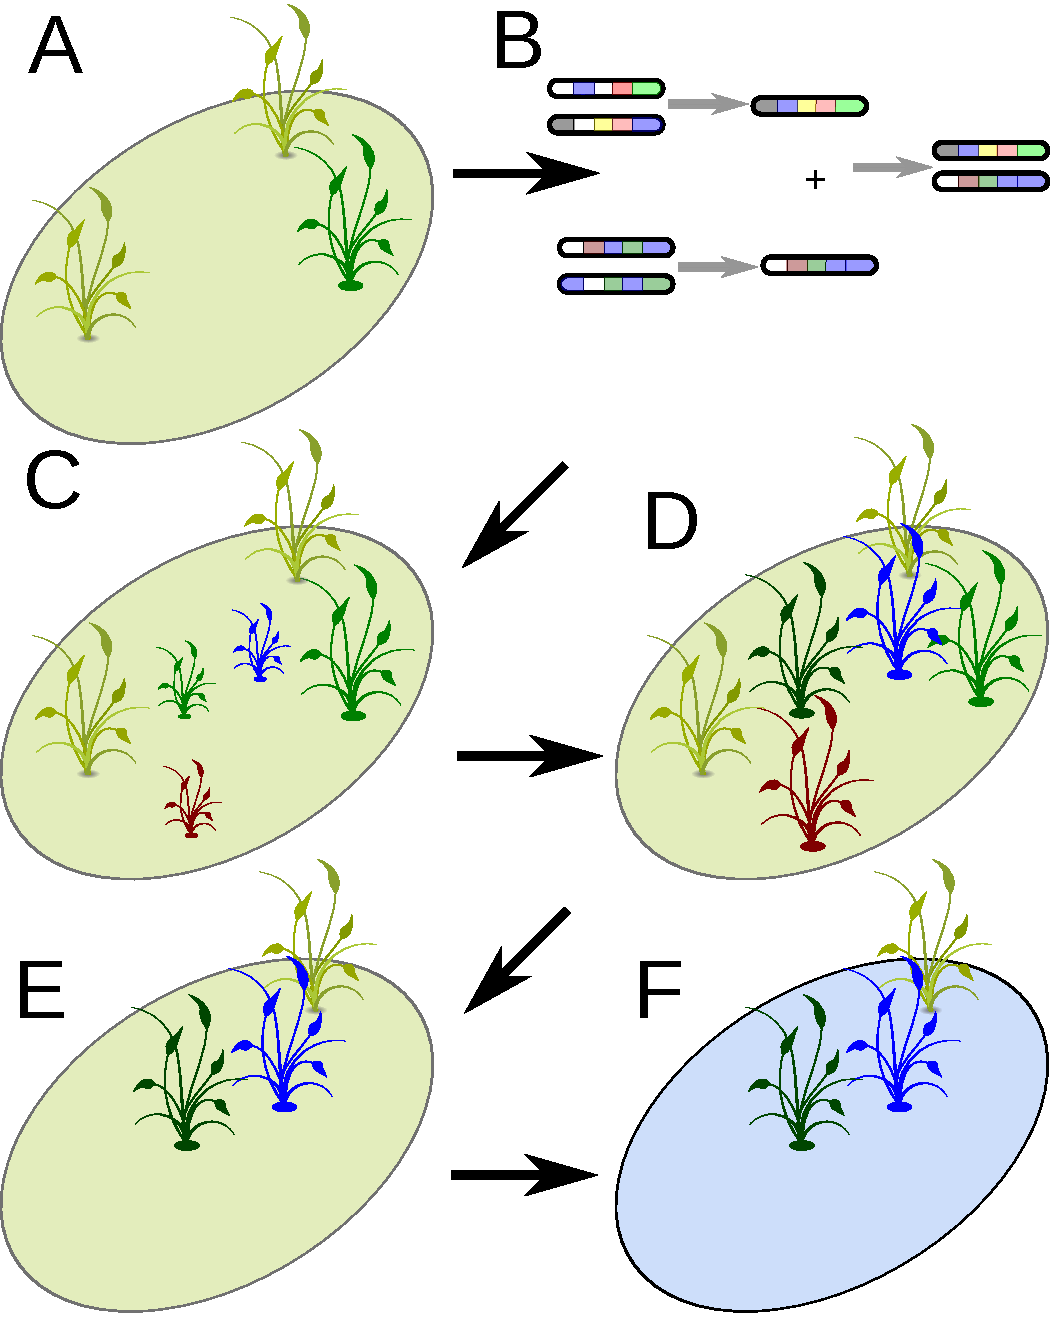
\includegraphics[width=0.6\linewidth] {MainTextFigures/Fig1.pdf}
\caption*{Figure 1. Calculations performed in sPEGG during each time step. Parents are identified (A), and genetic information is transmitted to offspring by subroutines implementing recombination and mutation (B). User-supplied functions map the resulting phenotypic distribution to newborns (C). A selective environment (here, substrate color in each panel) updates individual phenotypes (including mortality risk) (D) and survivors are identified (E). The relevant environmental variables variables are updated to reflect the phenotype distribution (F), thereby closing the eco-evolutionary feedback loop. Though not illustrated, gene flow resulting from migration among patches can also be modelled in sPEGG.}
\end{figure}

In sPEGG, the following calculations are performed at each step on each individual in each of the $n$ species. First, the eligible parents are identified according to rules supplied by the user, and the number of neonates are determined (Fig 1A). Second, parents are assigned to neonates, and genetic information is transmitted from the assigned parents to their offspring (Fig 1B). Third, based on the genetic information, the offspring's phenotype at birth is determined, based on a user-supplied genotype-phenotype map (Fig 1C). We highlight that sPEGG allows users to specify any genotype-phenotype map. Thus, in addition to an additive effect among loci, non-additive genetic effects such as dominance and epistasis, as well as maternal effects, environmental effects and gene $\times$ environment effects which characterize the trait of interest (\citealt{hendry13}) can be readily accommodated. Fourth, the individual's phenotypes (including their probability of survivorship) are updated according to the selective environment (which includes ecological interactions) that the user specifies (Fig 1D). Fifth, the survivors are identified and dead individuals are removed from the model (Fig 1E). A further step may involve updating the prevailing environmental conditions according to the phenotypic distribution of survivors, thereby completing the eco-evolutionary feedback loop (Fig 1F). The ability to simulate migration and gene flow in spatially-structured environments is also supported. sPEGG could be viewed as analogous to a numerical ordinary differential equation solver. As in those solvers, sPEGG still requires the user to provide some code describing the species-specific calculations, but the core computations above are carried out by the software. The online Methods describe sPEGG's design in greater detail.

sPEGG accommodates alternative mating systems (random, shared preference across individuals, or assortative;  monogamy or polygynandry). The transfer of genetic information can mimic recombination and sexual reproduction in diploid species or asexual reproduction, and can involve mutation and arbitrary linkage patterns. Importantly, all of these calculations, and more, are done across individuals using parallel algorithms, as described in the online Methods.

To illustrate the versatility and performance benefits of sPEGG, we use it to build IBMs to investigate three classic problems in evolutionary ecology. We first consider a very simple model of a randomly mating, diploid species with overlapping generations, in which the per-capita density-independent birth and death rate are quantitative traits whose numerical values are determined additively by five independently segregating loci subject to mutation in their allelic values (case study 1). Here, the population simply evolves to minimize density-independent mortality and maximize the density-independent birth rate (Supplementary Figure S1). Figure 2A shows that, as more individuals are simulated the total simulation speed increases approximately 10-fold compared to an equivalent simulation running entirely on a single CPU core.

\begin{figure}[h!]
   \centering
   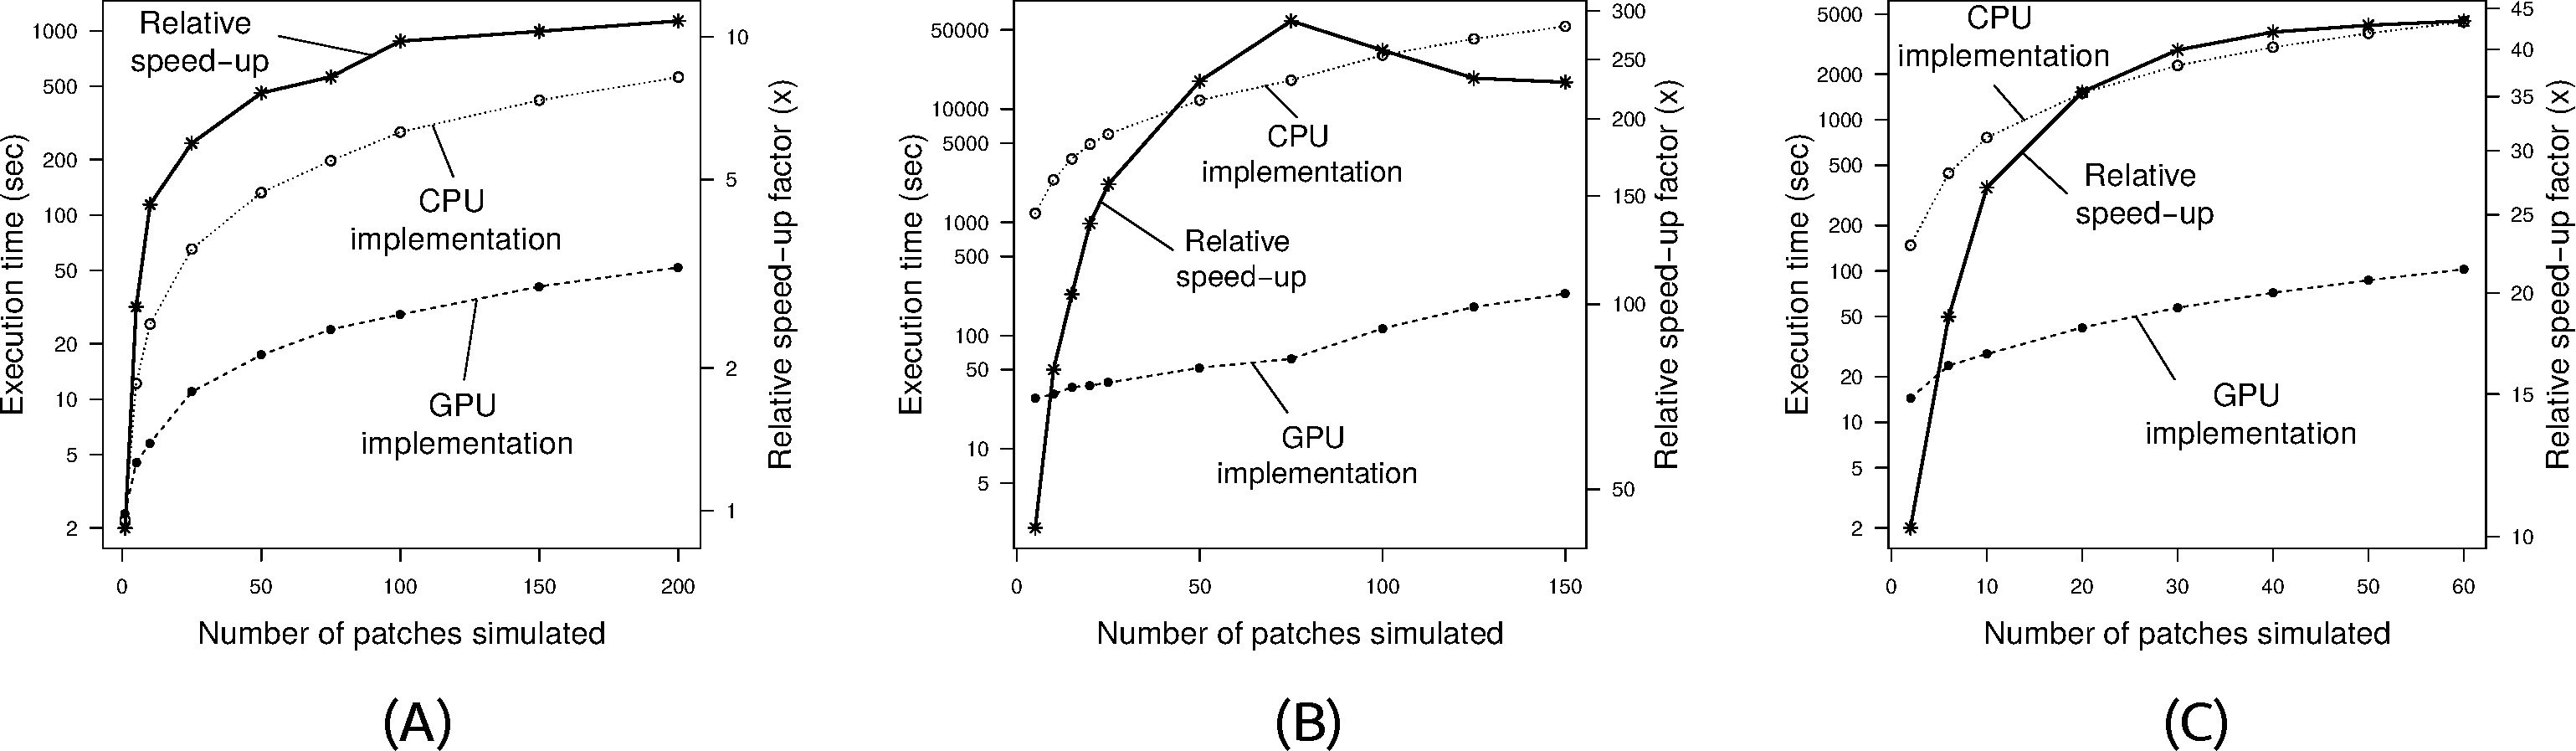
\includegraphics[width=\linewidth] {MainTextFigures/Fig2.pdf}
\caption*{Figure 2. Performance comparisons as functions of the problem size (number of patches simulated) in terms of the number of seconds it takes to execute the simulations for the CPU version of sPEGG (dotted lines, open circles) and the GPU version (dashed lines, filled circles), as well as the speed up of sPEGG relative to a serial implementation (solid lines, asterisks). Performance comparisons are based on 250 iterations of steps represented in Figure 1 in the main text for both implementations. (A) Results from case study 1, which models evolution in fecundity and density-independent survivorship. (B) Results from case study 2, which models the evolution of neonate size in a physiologically structured model for a species that experiences an ontogenetic niche shift. (C) Results from case study 3, which models coevolving consumer-resource metacommunities linked by migration. In all panels, each patch contains approximately 50,000 individuals of each species; thus, a simulation of 100 patches simulates approximately $5\times10^6$ individuals in (A), (B) and approximately $10^7$ individuals in (C).}
\end{figure}

Next, we use sPEGG to model a size- and physiologically-structured (e.g., \citealt{persson98}), sexually reproducing species in which individuals of different sizes complete for two dynamic, biological resources (case study 2). Individuals transition from utilizing one resource type to utilizing another as they increase in size. We model the evolution of offspring size at birth, a trait which we assume (i) is inversely related to clutch size, and (ii) is controlled additively by a finite number of loci. Offspring size is then modeled to evolve to maximize individual fitness, subject to the individual-level constraints of size-specific survivorship, resource-use, and fecundity (Supplementary Information S2). Figure 2B illustrates how when the evolutionary question is addressed by a complex IBM, sPEGG can accelerate the simulation on a GPGPU by a factor of over 200x.

As a final case study, we model a spatially-structured, consumer-resource system in which the resource species and the consumer species coevolve (case study 3). We also model anti-predator defense to be costly for the resource. We apply sPEGG to analyze coevolution in such a system, investigating how a spatial gradient in the cost of anti-predator defense drives coevolutionary dynamics (Supplementary Information S3). Figure 2c shows that the performance improvements provided by sPEGG are higher for case study 3 than for case study 1 (up to approximately a factor of 44x), and not as high as the performance improvements for case study 2. 

The GPGPU versions of all case studies show accelerations of up to 1-2 orders of magnitude compared to the serial implementations. The differences in performance between the case studies reflect differences in their biological complexity. The fraction of the code's execution time spent performing calculations evaluating fitness, as opposed to reading and writing data from memory (albeit within the confines of GPU memory), is higher for case studies 2 and 3 than for case study 1 (where the speed of the simulation is limited instead by the speed of memory access). We note, however, that even in complicated IBMs, memory access may eventually prove increasingly taxing as more patches are simulated (Fig. 2B). Our comparative analysis of the three case studies thus identifies the biological circumstances under which sPEGG is likely to be significantly more efficient than serial implementations.   

Our results show that the performance-improvements provided by sPEGG can best be exploited when calculating how ecological processes affect individual fitness, delivering performance improvements comparable to a small cluster for our most complicated case-study model. In addition to being the first general framework for constructing and accelerating evolutionary individual-based models on GPGPUs, sPEGG also represents the first resource using a generalized, forward time population genetics model to study multi-species evolution in ecological communities. Thus, sPEGG may be an especially attractive framework for using system-specific, mechanistic models to elucidate the interplay between ecological and evolutionary dynamics. 

\end{linenumbers}
\section*{Acknowledgments}
This research was funded in part by a Chair's Fellowship from the Department of Ecology and Evolutionary Biology at the University of California, Los Angeles to K.W.O and a Complex Systems Scholar Award from the James S. McDonnell Foundation and  NSF grant  DEB 1457815 to P.A. We would like to thank G. Lin for discussion and assistance with some of the programming. 

\bibliographystyle{cbe}	
\bibliography{myrefs11}
\newpage 

\section*{Supplementary Material}
Supplementary Figure S1. The evolutionary trajectory of the traits modeled in case study 1.

\noindent Supplementary Information S2. Description of eco-evolutionary model used in case study 2.

\noindent Supplementary Information S3. Description of eco-evolutionary model used in case study 3.

\noindent Supplementary Figure S4. Description of the species class used in sPEGG models.

\noindent Supplementary Figure S5. Pseudo-code illustrating the difference between the serial  and parallel implementations of individual-based models in sPEGG. 

\end{document} 
